\documentclass[border=10pt]{standalone}
\usepackage{xcolor}
\usepackage{tikz}
\usetikzlibrary{fit,backgrounds,positioning}

\definecolor{INK}{HTML}{1A1A2E}
\definecolor{BG}{HTML}{FAFAFA}
\definecolor{SUB}{HTML}{555566}
\definecolor{COLD}{HTML}{4361EE}
\definecolor{WARM}{HTML}{2EC4B6}

\begin{document}
\pagecolor{BG}
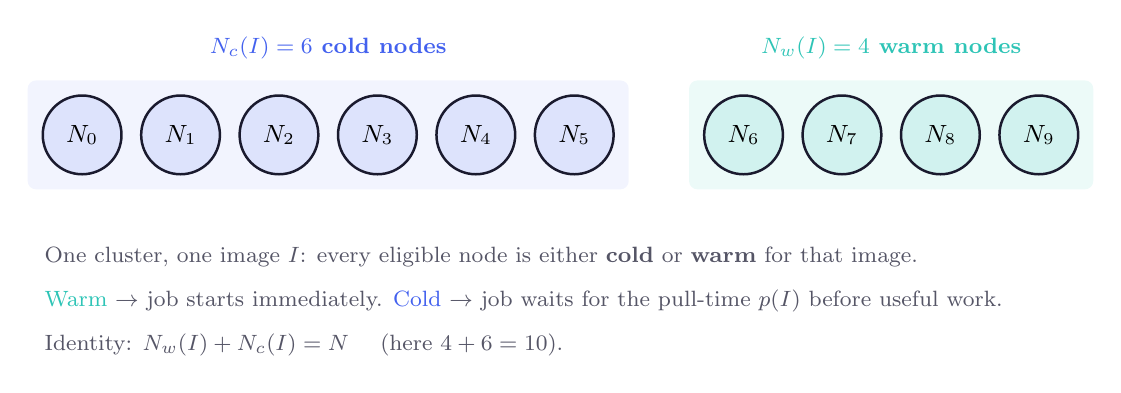
\begin{tikzpicture}[
    font=\sffamily,
    nd/.style={circle, draw=INK, line width=0.9pt, minimum size=10mm, inner sep=0pt, font=\small\bfseries},
    cold/.style={nd, fill=COLD!18},
    warm/.style={nd, fill=WARM!22},
    caplbl/.style={font=\footnotesize\bfseries},
    sub/.style={font=\footnotesize, text=SUB},
  ]

  % cold nodes
  \foreach \i in {0,...,5} {
    \node[cold] (c\i) at (\i*1.25, 0) {$N_\i$};
  }
  % warm nodes
  \foreach \i [evaluate=\i as \x using (\i-6)*1.25 + 8.4] in {6,...,9} {
    \node[warm] (w\i) at (\x, 0) {$N_\i$};
  }

  % group brackets
  \begin{scope}[on background layer]
    \node[fill=COLD!7, rounded corners=3pt, fit=(c0)(c5), inner sep=5pt] (coldbox) {};
    \node[fill=WARM!9, rounded corners=3pt, fit=(w6)(w9), inner sep=5pt] (warmbox) {};
  \end{scope}

  \node[caplbl, text=COLD, above=4pt of coldbox] {$N_c(I)=6$ cold nodes};
  \node[caplbl, text=WARM, above=4pt of warmbox] {$N_w(I)=4$ warm nodes};

  % bottom explanation
  \node[sub, anchor=north west] at (-0.6, -1.3)
    {One cluster, one image $I$: every eligible node is either \textbf{cold} or \textbf{warm} for that image.};
  \node[sub, anchor=north west] at (-0.6, -1.85)
    {\textcolor{WARM}{Warm} $\rightarrow$ job starts immediately. \textcolor{COLD}{Cold} $\rightarrow$ job waits for the pull-time $p(I)$ before useful work.};
  \node[sub, anchor=north west] at (-0.6, -2.4)
    {Identity: $N_w(I) + N_c(I) = N$ \quad (here $4 + 6 = 10$).};

\end{tikzpicture}
\end{document}
